\section{\texorpdfstring{ 面向多标签眼科疾病识别的可解释与隐私保护单域泛化(Interpretable Single Domain Generalization with Privacy-Preserving for Multi-Label Ocular Disease Recognition)}{ 面向多标签眼科疾病识别的可解释与隐私保护单域泛化(Interpretable Single Domain Generalization with Privacy-Preserving for Multi-Label Ocular Disease Recognition)}}\label{ux9762ux5411ux591aux6807ux7b7eux773cux79d1ux75beux75c5ux8bc6ux522bux7684ux53efux89e3ux91caux4e0eux9690ux79c1ux4fddux62a4ux5355ux57dfux6cdbux5316interpretable-single-domain-generalization-with-privacy-preserving-for-multi-label-ocular-disease-recognition}

\subsection{摘要}\label{ux6458ux8981}

深度学习在早期眼底疾病诊断分析中潜力巨大，能帮助患者预防不可逆视力丧失，但实际应用中面临多重挑战：单域训练模型跨医疗机构时，常因成像设备、光照和人群差异引发域偏移，导致泛化性能下降；临床中单眼多疾病共存，标准分类器易误判或漏检；医疗数据高度敏感，传统DA方法在多域暴露场景下存在隐私机制添加复杂、性能衰减严重问题。针对这些挑战，我们设计双分支引导单域泛化（SDG）框架，仅用单一域数据结合类别激活映射图(CAM)引导训练，提取单域域不变特征，实现对未知域的适应，同时CAM图提供关注区域可视化，增强可解释性。为解决多标签分类难题，我们嵌入Transformer机制建模标签关联性，捕捉疾病共现依赖，减少误检漏检。对于跨域场景下隐私防护难问题，我们探索出了一种跨域与隐私保障兼得的方案：在单域泛化SDG训练过程中，集成高斯差分隐私，通过梯度噪声注入，能在中等隐私保护下性能接近基线。综合以上，我们搭建了一个具有隐私保护的多标签眼病识别可解释单域泛化框架。在实验部分，通过完整的消融实验分析证明该框架有效可靠，跨域表现优异，且隐私模式下性能衰减可控。

\subsection{关键词: Domain Generalization; Multi-Label Ocular Disease Recognition; Data Privacy; Interpretability}\label{ux5173ux952eux8bcd-domain-generalization-multi-label-ocular-disease-recognition-data-privacy-interpretability}

\subsection{1.引言}\label{ux5f15ux8a00}

深度学习技术作为人工智能的核心，已在图像处理领域广泛应用，主要包括图像分类\hyperref[_Ref213871637]{{[}1{]}}、语义分割\hyperref[_Ref213948625]{{[}2{]}}、图像生成\hyperref[_Ref213948646]{{[}3{]}}以及超分辨率重建\hyperref[_Ref213948898]{{[}4{]}}等。在医疗领域，深度学习扩展到了许多横向应用，如疾病诊断与预测\hyperref[_Ref213949262]{{[}5{]}}，药物研发\hyperref[_Ref213949290]{{[}6{]}}，医学报告生成\hyperref[_Ref213949294]{{[}7{]}}等。这些应用利用深度学习的端到端学习能力，能处理多模态医疗数据，提高诊断效率和准确性。进一步聚焦于眼科疾病识别领域，早期眼底筛查是识别眼科疾病的关键技术之一\hyperref[_Ref213949315]{{[}8{]}}，深度学习通过分析眼底图像可及时发现潜在问题，帮助患者避免不可逆的视力丧失。然而，目前深度学习方法在医疗领域直接应用仍面临诸多挑战，包括跨域应用时的域偏移、临床多疾病共存条件下的疾病误判或漏检率高，以及医疗数据隐私易暴露。具体而言：

1.深度学习的模型性能取决于训练数据的数据量。在自然图像领域，数据收集相对简单，标注成本较低，因此涌现了许多经典数据集，如ImageNet\hyperref[_Ref213949336]{{[}9{]}}和COCO\hyperref[_Ref213949340]{{[}10{]}}等。然而，医疗领域数据与自然图像不同，医疗数据集的标注需由专业医生完成，以确保质量和可靠性，这个过程费时费力。另外，即使通过某个医疗机构的源域数据集训练得到了一个性能良好的模型，将其应用到另外的机构时，目标域的数据常因成像设备、光照和人群差异引发域偏移gap\hyperref[_Ref213949348]{{[}11{]}}，导致模型性能下滑，如图a1和a3所示，源域和目标域的分布有差异，用源域训练的base模型(\hl{图1.b1})得到的决策边界可能不适用于目标域分布(\hl{图1.b2})。常见的消除gap的方法如域适应方法DA选择将源域和目标域数据一同送入模型训练来对齐域分布\hyperref[_Ref213949354]{{[}12{]}}，使得决策边界可以复用。但是在实际应用中，由于医院和患者之间的保密性，大部分的数据集是不公开的，所以可能难以获取到目标域数据集用于域适应。因此探索一种单域训练来找到更鲁棒的决策边界的方法可能更适用于以上场景。

\begin{center}
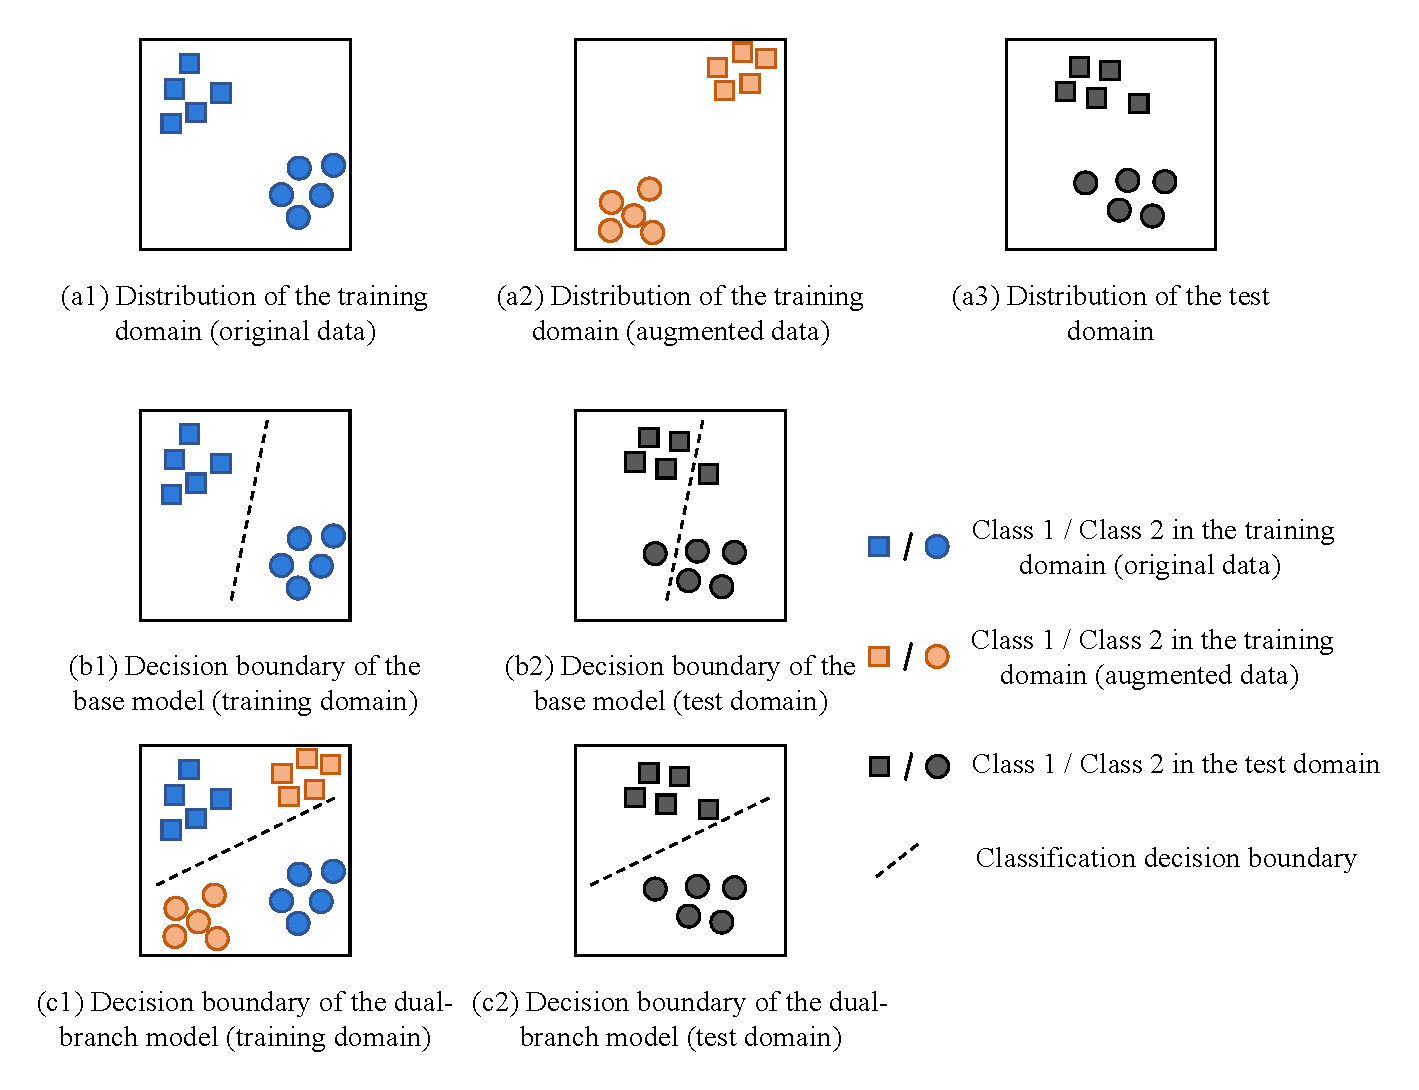
\includegraphics[width=0.72\textwidth]{./images/media/image1_padded.pdf}
\end{center}

2.在图像处理领域，单标签识别的数据集和任务占多数，所以此方面的研究较多，性能也在不断提高。但是将这些方法应用到眼底疾病识别任务上有局限性。因为临床条件下，单眼可能存在多疾病共存，若常规方法进行疾病识别，误判和漏检现象严重\hyperref[_Ref213949362]{{[}13{]}}。近年来，自然图像中也存在多标签识别方法的相关工作，比如ML-GCN \hyperref[_Ref213949382]{{[}14{]}}，通过统计各标签出现的频率建立图关联性，使得识别出某个标签后，更有可能识别出其关联标签，从而减少漏检。而在眼底多标签疾病识别中，各疾病之间的关联性更加错综复杂，仅靠标签频率来建立疾病关联性的方法对于这种复杂情况效果可能不可靠。因此针对眼底多标签识别探索一种更高效可靠的疾病关联性构建方法成为可能。

3.医疗数据比起自然图像特殊，存在数据隐私问题，且在传统的域适应跨域场景下更为严重。常见的攻击方法可以通过模型的训练梯度逆向恢复出患者的数据\hyperref[_Ref213949393]{{[}15{]}}。针对此问题，目前存在相关的隐私保护方法研究，但是都存在trade-off问题：隐私保护和性能良好不可兼得，且应用到da场景时尤为明显，可能存在隐私机制添加复杂，两域性能衰减严重等问题。因此需要在跨域场景探索出一种隐私保护和跨域性能平衡的方法。

为应对上述三个关键挑战，我们构建了一个融合隐私保护的多标签眼科疾病分类可解释框架。针对跨域泛化难题，我们提出双分支引导的域不变特征提取模块，仅利用单一源域数据进行训练，框架通过对训练域原始图像及其分布扰动后的增强图构建双分支结构（如图 1.a1 和图 1.a2 所示），在特征层面显式挖掘两者的共有表示。同时，引入基于 CAM 的类别关注区域作为先验引导，促使模型聚焦于疾病相关区域，从而抑制域特定噪声特征的学习，使得模型能够形成更鲁棒的决策边界（图 1.c1），并在未知测试域上保持稳定的分类性能（图 1.c2）。此外，CAM 热图还为模型预测提供了直观的关注区域可视化，增强了模型的可解释性；针对眼科场景中普遍存在的多疾病共现问题，我们引入基于 Transformer 的标签--特征关联性建模模块，过自注意力建模标签间的内在关联关系，并利用交叉注意力将标签语义与对应的图像特征进行融合，在标签层面与特征层面同时构建疾病共现依赖，从而有效减少多标签识别中的误检与漏检；针对跨域医疗场景下的数据隐私风险，本文在单域泛化训练过程中集成高斯差分隐私机制，通过在梯度更新阶段注入噪声实现隐私保护。在中等隐私预算条件下，该机制能够在不显著牺牲模型性能的前提下提供有效的隐私保障，实现跨域泛化能力与数据隐私保护的兼顾。

最后在多个具有代表性的眼底影像数据集和跨站点测试设置上进行的系统实验表明，该框架在保持良好可解释性的同时，在跨域多标签分类性能与隐私约束条件下均展现出稳定且优越的表现。

我们贡献如下：

1.设计了一种双分支引导域不变特征提取模块（Dual-branch guided Domain-invariant Feature Extraction, DFE），通过分布扰动增强与类别激活映射（CAM）联合引导，显式抑制域特定噪声特征，强化疾病相关判别信息，不仅提升了跨域泛化性能，同时增强了模型预测的可解释性。

2.提出了一种自适应标签--特征关联性构建模块（Adaptive label-feature Relevance Construction, ARC），基于 Transformer 的自注意力与交叉注意力机制，在标签层面与特征层面同时建模疾病共现依赖，有效降低了多标签眼科疾病识别中的误检与漏检问题。

3.将自适应高斯差分隐私机制（Adaptive Gaussian Differential Privacy, AdaGDP）集成至单域泛化训练流程中，在不引入目标域数据的前提下，实现了隐私保护与跨域泛化性能之间的有效平衡，验证了在中等隐私预算条件下模型性能仍可接近非隐私基线。

本文的其余部分安排如下：第二节介绍了近年来的相关工作。 所提出方法的具体阐述于第三节介绍，第四节展示完整的实验设置和结果。第五节得出结论并展开未来工作的讨论。

\subsection{2.相关工作}\label{ux76f8ux5173ux5de5ux4f5c}

\subsubsection{A.域泛化}\label{a.ux57dfux6cdbux5316}

在计算机视觉任务中，模型在单一域上训练后应用于新域时，常因成像条件、光照或数据分布差异导致域间差距gap，从而性能下降。这种跨域差距在医疗成像中尤为突出，不同医院或设备的数据集间存在显著偏移，影响泛化能力\hyperref[_Ref213949439]{{[}16{]}}。常见的解决方法是域适应DA，通过在训练中对齐源域和目标域分布来缓解差距。例如基于最大均值差异MMD\hyperref[_Ref213949448]{{[}17{]}}对齐或相关性对齐（CORAL）\hyperref[_Ref213949453]{{[}18{]}}，能最小化分布差异，提高迁移性能； DANN\hyperref[_Ref213949479]{{[}19{]}}采用对抗训练机制迷惑域分类器，学习域不变特征，在数字识别等任务中实现鲁棒转移；其他DA方法如如CycleGAN\hyperref[_Ref213949490]{{[}20{]}}使用循环一致生成对抗网络进行无配对图像风格转换，可以有效桥接域间风格差异，尤其适用于无监督场景\hyperref[_Ref213949530]{{[}21{]}}。

然而，DA需要训练时访问目标域数据，这在隐私场景或访问受限场景下不切实际。近年来，域泛化DG作为更实用的替代方案流行起来，仅在单个或者多个源域上训练学习不变表示，泛化到未知目标域\hyperref[_Ref213949554]{{[}22{]}}。DG在无需目标数据的情况下优于DA，强调多源鲁棒性。典型方法包括MixStyle\hyperref[_Ref213949562]{{[}23{]}}，通过混合实例风格统计模拟域偏移，提升不变性；DomainBed\hyperref[_Ref213949607]{{[}24{]}}提供多域基准，用于评估DG算法在多样数据集上的表现；Fact\hyperref[_Ref213949788]{{[}25{]}}利用傅里叶变换，将特征分解为域特定和不变组件，利用振幅混合和联合教师正则化机制进行泛化；RSC \hyperref[_Ref213949796]{{[}26{]}}丢弃主导特征，迫使网络激活剩余的与标签相关的特征促使泛化；基于元学习的DG\hyperref[_Ref213949803]{{[}27{]}}通过 episodic 训练模拟偏移。在医疗领域，这些DG技术在跨设备MRI、CT影像分类应用中\hyperref[_Ref213949863]{{[}28{]}}，可以避免目标数据依赖，提升分布外性能。

\subsubsection{B.多标签图像识别}\label{b.ux591aux6807ux7b7eux56feux50cfux8bc6ux522b}

不同于单标签多分类任务，多标签多类图像识别限制更为宽泛，前者需要为图像分配互斥类别\hyperref[_Ref213949872]{{[}29{]}}，而后者可以为单图像分配多个标签。因此多标签图像识别任务更复杂，需要捕捉共现类别、处理标签依赖和不平衡问题，通常使用二元交叉熵损失而非softmax。这种复杂性源于标签间相关性，忽略关联会导致不完整预测。

在自然图像领域，多标签识别方法早期如Binary Relevance\hyperref[_Ref213949896]{{[}30{]}}将问题视为独立二元分类，但忽略相关性。更先进方法融入标签依赖，如 ML-GCN，从标签共现统计构建图传播信息，在COCO数据集上提升性能；Asymmetric Loss (ASL)\hyperref[_Ref213949927]{{[}31{]}} 通过不对称方式调整正负样本的权重,处理样本不平衡问题, 引入概率移位机制,避免模型过度拟合噪声信息；基于Transformer的Query2Label\hyperref[_Ref213950246]{{[}32{]}}使用查询(query)建模标签交互，通过注意力在VOC\hyperref[_Ref213950282]{{[}33{]}}和COCO上达到最优。这些方法利用大规模自然图像数据集学习丰富表示，通过语义嵌入减少误检。在医疗成像中，多标签图像识别尤为关键，因为疾病往往共存，忽略标签间相关性可能导致临床诊断错误。典型方法包括MulGCN\hyperref[_Ref213950338]{{[}34{]}}，将疾病关系建模为图，使用两个连体图卷积网络（GCN）分别处理节点特征和标签表征，捕捉共现关系并传播信息，以提升多标签预测的准确性；基于注意力的多尺度MobileNet\hyperref[_Ref213950343]{{[}35{]}}，通过融合多尺度特征并引入注意力模块突出关键区域，处理眼底图像中的疾病共现和不平衡标签. 实现了高效的多标签眼科疾病检测；FedMLP\hyperref[_Ref213950349]{{[}36{]}}，一种两阶段联邦学习框架，用于任务异构下的多标签医疗图像分类，通过伪标签标记为未标注数据生成可靠的多标签指导，并结合全局知识蒸馏捕捉标签依赖关系，从而处理不平衡和共现问题。这些方法强调领域特定适应，有效管理复杂医疗标签依赖和不平衡问题。

\subsubsection{C.隐私保护}\label{c.ux9690ux79c1ux4fddux62a4}

近年来，隐私问题日益突出，尤其在医疗领域，患者图像和记录等敏感数据在AI训练中易遭泄露\hyperref[_Ref213950358]{{[}37{]}}。医疗数据共享可能违反HIPAA或GDPR法规，模型通过记忆或推理攻击泄露信息。常见解决方法包括联邦学习FL，在分布式设备上本地训练模型，无需集中数据\hyperref[_Ref213950376]{{[}38{]}}。例如，FedAvg\hyperref[_Ref213950381]{{[}39{]}}聚合客户端更新构建全局模型，在医疗如COVID-19检测中保护隐私；FedProx\hyperref[_Ref213950391]{{[}40{]}}添加近端项处理异构数据，提升医疗FL稳定性。

同时，为进一步防范隐私泄露，加密机制提供更强保障。同态加密HE\hyperref[_Ref213950427]{{[}41{]}}允许加密数据上计算，无需解密，适用于多方医疗分析，但计算开销大\hyperref[_Ref213950433]{{[}42{]}}；安全多方计算SMPC\hyperref[_Ref213950438]{{[}43{]}}联合计算保持输入隐私，在协作诊断中优势明显。差分隐私DP\hyperref[_Ref213950443]{{[}44{]}}通过向查询或梯度添加噪声界定泄露风险，提供量化保证（如\(\epsilon\)-DP）；高斯DP\hyperref[_Ref213950449]{{[}45{]}}作为更松弛的变体，使用高斯噪声平滑隐私-效用权衡，在医疗成像中防护成员推理攻击。其他机制包括Trusted Execution Environments (TEE)\hyperref[_Ref213950453]{{[}46{]}}如Intel SGX，在安全硬件隔离中计算，云医疗AI隐私强。DP在深度学习梯度保护中突出，但在多域设置下容易造成准确性下降\hyperref[_Ref213950458]{{[}47{]}}，所以需要思考如何平衡隐私与性能。

\subsection{3.提出的方法}\label{ux63d0ux51faux7684ux65b9ux6cd5}

所提出的面向多标签眼科疾病分类的可解释单域泛化框架概述图如图2所示，分为两个主要部分：Part1.双分支引导域不变特征提取，Part2.自适应标签-特征关联性构建。Part1的作用是以疾病CAM图引导模型学习，结合双分支对比学习，提取单域的疾病相关特征，减少噪声特征学习，使决策边界更鲁棒，便于泛化到其他域，同时CAM图可提供模型决策时的关注区域可视化，增强可解释性。在保证Part1的域不变特征提取的基础上，Part2通过注意力机制建立标签与标签、标签与特征间的关联性，解决多标签分类中的误检漏检问题。最终将双分支的各注意力向量计算特征一致性，由此提升多标签识别的单域泛化能力。另一方面，为了保证隐私，训练过程中添加高斯差分隐私机制，追求隐私-性能间的效益平衡。综合以上，所提出的方法构建了一个具有隐私保护的多标签眼病识别可解释单域泛化框架。以下分三小节详细描述各模块的实现细节。

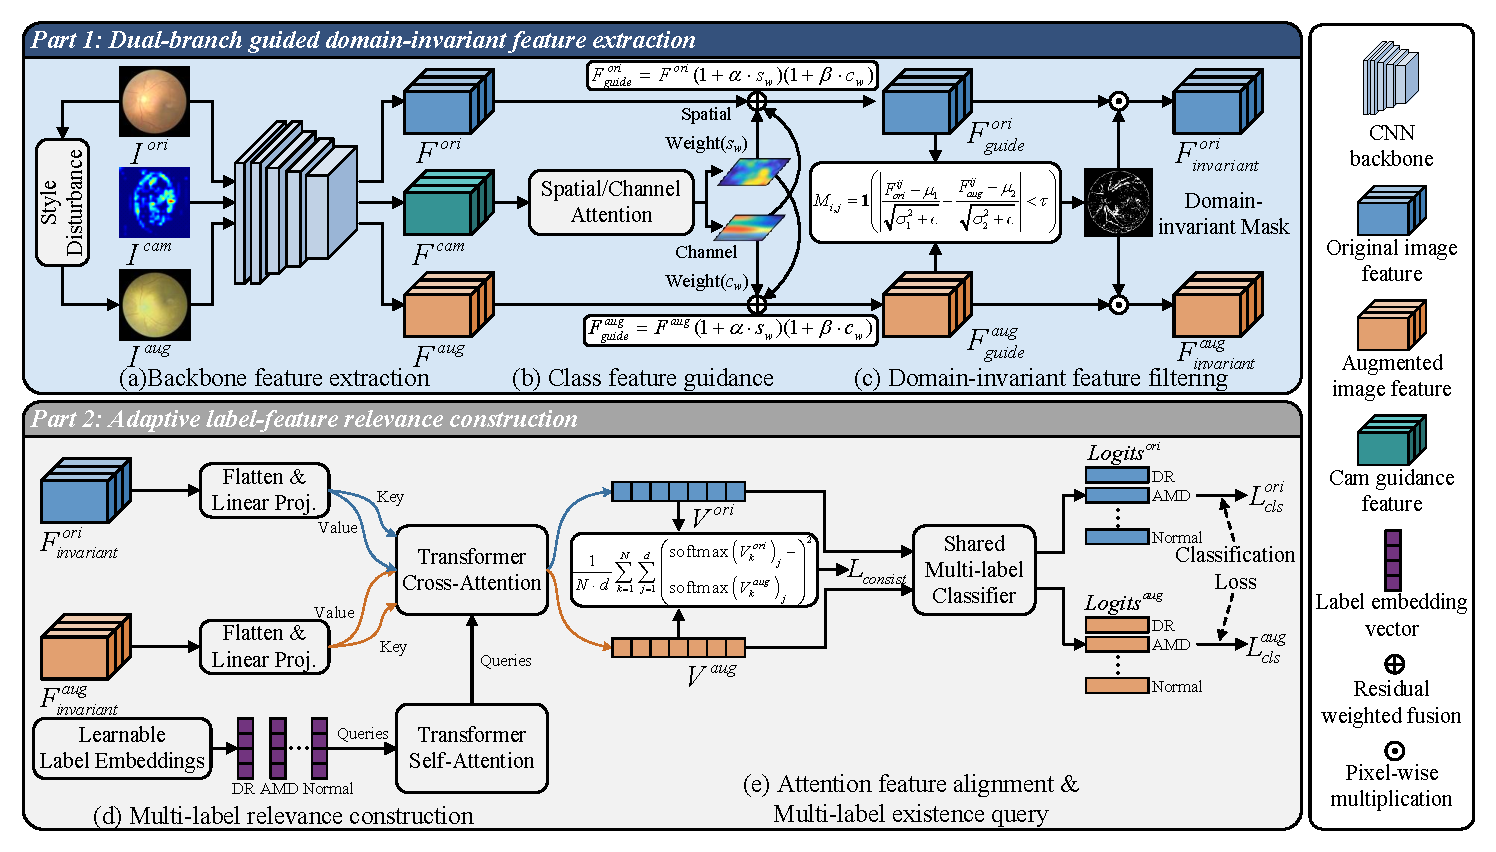
\includegraphics[width=5.76458in,height=3.21181in]{./images/media/image2_padded.pdf}

A.双分支引导域不变特征提取

训练域只有单域数据，但其中存在可泛化到其他域的域不变信息，若能有效提取，可以实现对未知域的鲁棒泛化。受对比学习启发，将原图利用风格扰动等增强技术创建增强图，用于模拟未知域可能出现的各种分布差异。具体而言，原图\(I_{ori}\)代表训练域的原始眼底图像，而增强图\(I_{aug}\)通过风格扰动（如MixStyle方法或随机调整亮度、对比度、饱和度）生成。这种增强模拟了跨域场景中的成像设备、光照环境或患者群体差异，但保留了图像的语义内容（疾病病变区域）。

首先，如图2(a)部分所示，\(I^{ori}\)和\(I^{aug}\)二者共同送入骨干网络提取特征得到\(F^{ori}\)和\(F^{aug}\)。令\(F^{ori} \in \mathbb{R}^{C \times H \times W}\)和\(F^{aug} \in \mathbb{R}^{C \times H \times W}\)，其中\(C\)、\(H\)、\(W\)分别为骨干网络的最终特征图尺寸通道数、高度和宽度。本方法选择ResNet-50作为骨干网络，因为其在医疗图像分类中表现出色，具有较好的特征提取能力和计算效率。然而，仅靠\(F^{ori}\)和\(F^{aug}\)的对比学习效果有限，因为在提取域不变信息的同时，模型可能会学到噪声特征（如背景纹理或无关光影），这些噪声会干扰决策边界，导致泛化性能下降。

为此，我们引入图2(b)部分的类别特征引导模块，以提升特征的疾病相关性和可解释性。预先使用基线模型（ResNet-50 + BCE损失）在训练集上生成类激活图（CAM）。CAM突出模型对不同疾病区域的关注，例如糖尿病视网膜病变（DR）关注血管区，年龄相关性黄斑变性（AMD）关注黄斑区。其计算公式为：

\[I^{cam} = \sum_{k = 1}^{C}w_{k} \cdot A_{k},
\]

其中\(A_{k}\)是骨干网络最后一层卷积的第\(k\)个通道激活图，\(w_{k}\)是通过全局平均池化后对分类权重的梯度计算得到的权重。该公式基于Grad-CAM变体，确保CAM捕捉类别特定关注区域。生成的CAM热图\(I^{cam}\)输入骨干网络得到\(F^{cam} \in \mathbb{R}^{C \times H \times W}\)，然后通过空间/通道注意力模块分别计算\(F^{cam}\)的空间注意力权重\(s_{w}\)和通道注意力权重\(c_{w}\)。两个注意力模块均为卷积序列网络，都包含有1x1卷积、ReLU激活和Sigmoid函数，用于自适应生成权重。空间注意力模块额外结合平均/最大池化捕捉局部上下文，从而生成像素级权重图，自适应放大病变区域（如血管或黄斑）的显著性，同时抑制背景噪声。通道注意力模块则采用自适应平均池化压缩空间维度以获取全局统计，随后学习通道依赖，从而增强疾病纹理敏感通道的权重，抑制噪声通道。分别将两权重加权应用到\(F^{ori}\)和\(F^{aug}\)得到cam引导特征\(F_{guide}^{ori}\)和\(F_{guide}^{aug}\)，具体的加权方式采用残差连接机制，避免过度引导破环原始信息。公式为：

\[F_{guide}^{ori} = F^{ori}(1 + \alpha{\cdot s}_{w})(1 + {\beta \cdot c}_{w}),
\]\[F_{guide}^{aug} = F^{aug}(1 + \alpha{\cdot s}_{w})(1 + {\beta \cdot c}_{w}),\]

其中\(\alpha\)和\(\beta\)分别为控制\(s_{w}\)和\(c_{w}\)增强程度的超参数。残差加权方式确保了CAM引导提供疾病特征的关联信息，使模型训练时更有方向性，减少噪声信息的学习，提高了其域不变特征与噪声特征的对比度。在此基础上再提取域不变特征效果更好，同时CAM热图的可视化直接增强了模型的可解释性，帮助临床医生理解预测依据，例如通过叠加热图观察模型是否关注正确病变区。

接下来是双分支域不变特征提取方法，如图2(c)部分所示，我们采用mask掩码方法，思路为将原图引导特征和增强图引导特征在特征分布层面计算相似度，相似度高的部分（域不变）保留，低的部分（域特定噪声）剔除。掩码矩阵\(M \in \mathbb{R}^{C \times H \times W}\)的计算基于标准化距离：

\[
M_{ij} =
\left\{
\begin{array}{ll}
1, & \text{if } \left| \dfrac{F_{guide}^{ori,ij} - \mu_{1}}{\sqrt{\sigma_{1}^{2} + \epsilon}} - \dfrac{F_{guide}^{aug,ij} - \mu_{2}}{\sqrt{\sigma_{2}^{2} + \epsilon}} \right| \leq \alpha, \\
0, & \text{otherwise.}
\end{array}
\right.
\]

其中\(\mu_{1},\sigma_{1}\)和\(\mu_{2},\sigma_{2}\)分别是两个引导特征的均值和方差，\(\epsilon = 10^{-5}\)为稳定性常数，\(i,j\)表示特征图位置。然后根据阈值\(\alpha\)将相似部分置1，不相似置0。最终将掩码矩阵分别应用到\(F_{guide}^{ori}\)和\(F_{guide}^{aug}\)提取域不变特征，具体为：

\[F_{invariant}^{ori} = F_{guide}^{ori} \odot M,F_{invariant}^{aug} = F_{guide}^{aug} \odot M,
\]

其中\(\odot\)是像素级逐元素乘法，确保只保留共有的疾病相关特征，如血管或黄斑区纹理，而剔除光照或设备噪声。此特征是Part2部分的基础。

B.自适应标签-特征关联性构建

多标签眼科疾病分类面临疾病共现挑战（如DR与AMD同时出现），传统方法忽略标签依赖易导致漏检。为了提高多标签识别性能，需要构建关联性。为此，嵌入Transformer注意力机制，在标签和特征层面构建相关性，实现自适应多标签预测。具体模块如图2(d)和(e)所示，包括多标签相关性构建和注意力特征对齐。

首先，将8类标签（ODIR数据集：正常、DR、AMD等）建模为可学习向量\(L = \lbrack L_{1},\ldots,L_{8}\rbrack \in \mathbb{R}^{8 \times d}\)，其中\(d = 512\)是嵌入维度。这些向量初始化为随机高斯分布，并在训练中优化，捕捉标签语义（如DR和AMD的共现概率）。标签向量输入到Transformer自注意力机制（Self-Attention），建模内部关联：

\[
V_{self} = softmax\left(\frac{QK^{T}}{\sqrt{d_{k}}}\right)V,
\]

其中\(Q = LW_{Q},K = LW_{K},V = LW_{V}\)，\(W_{Q},W_{K},W_{V}\)是可学习投影矩阵，\(d_{k} = d/heads\)（多头注意力，heads=8）。自注意力输出\(V_{self}\)捕捉标签依赖，该机制允许标签间动态交互，强化共现疾病的权重。

接下来，使用交叉注意力（Cross-Attention）将标签与域不变特征结合。因为Transformer需要接收序列输入，我们先将Part1输出的\(F_{invariant}^{ori}\)和\(F_{invariant}^{aug}\)展平（Flatten），作为Key和Value，与标签向量\(V_{self}\)作为Query，进行交叉注意力计算。计算公式为：

\[
V_{cross}^{ori} = softmax\left(\frac{V_{self}W_{Q}(F_{invariant}^{ori}W_{K})^{T}}{\sqrt{d_{k}}}\right)(F_{invariant}^{ori}W_{V}),
\]

类似计算\(V_{cross}^{aug}\)。通过多层交叉注意力机制，标签与对应疾病特征进行匹配，形成注意力向量\(V \in \mathbb{R}^{8 \times d}\)，突出疾病相关区域（如像素级乘法增强病变区）。由于自注意力机制各标签之间有关联，结果即为，查询出某个标签在图像的存在性之后，会增大概率检索其他关联标签的存在性，例如检测到DR后，更易激活AMD的查询。该设计在特征和标签层面同时构建疾病共现依赖，减少多标签识别的误检漏检。

为了确保双分支向量输出一致，我们引入注意力特征对齐模块，计算一致性损失。该损失使得在构建关联性的同时，不破坏原图和增强图向量的相似性，保留泛化性。具体计算方式为均方误差（MSE），公式为：

\[
L_{consist} = \frac{1}{N \cdot d}\sum_{k = 1}^{N}\sum_{j = 1}^{d}\left( softmax\left( V_{k}^{ori} \right)_{j} - softmax\left( V_{k}^{aug} \right)_{j} \right)^{2},
\]

其中\(N = 8\)是标签数，\(d = 512\)是嵌入维度，\(softmax\)确保概率分布一致。该损失强制分支间注意力向量对齐，提升模型在域偏移下的稳定性。

最终，注意力向量输入多标签分类器，首先对类别查询特征施加LayerNorm与Dropout以进行轻量级特征增强，以规范化和正则化查询特征，随后通过逐类别的线性变换获得每个类别的logits，经Sigmoid激活后，得到各类别的预测概率\(p^{ori}\)，类似得到\(p^{aug}\)。分类损失采用二元交叉熵（BCE）：

\[L_{cls}^{ori} = - \frac{1}{8}\sum_{k = 1}^{8}{\lbrack y_{k}\log p_{k}^{ori} + (1 - y_{k})\log(1 - p_{k}^{ori})\rbrack},
\]

总损失为\(L = L_{cls}^{ori} + L_{cls}^{aug} + \lambda L_{consist}\)，其中\(\lambda\)为平衡一致性程度的超参数。

C. 隐私保护集成

医疗图像数据高度敏感，训练过程中共享梯度易被梯度逆向攻击恢复原始图像，导致患者隐私泄露。为了在单域泛化框架中实现隐私与性能的有效平衡，我们引入自适应高斯差分隐私（Adaptive Gaussian Differential Privacy, AdaGDP）机制，相比传统的高斯差分隐私有显著改进。整体的隐私保护框架图如图3所示。

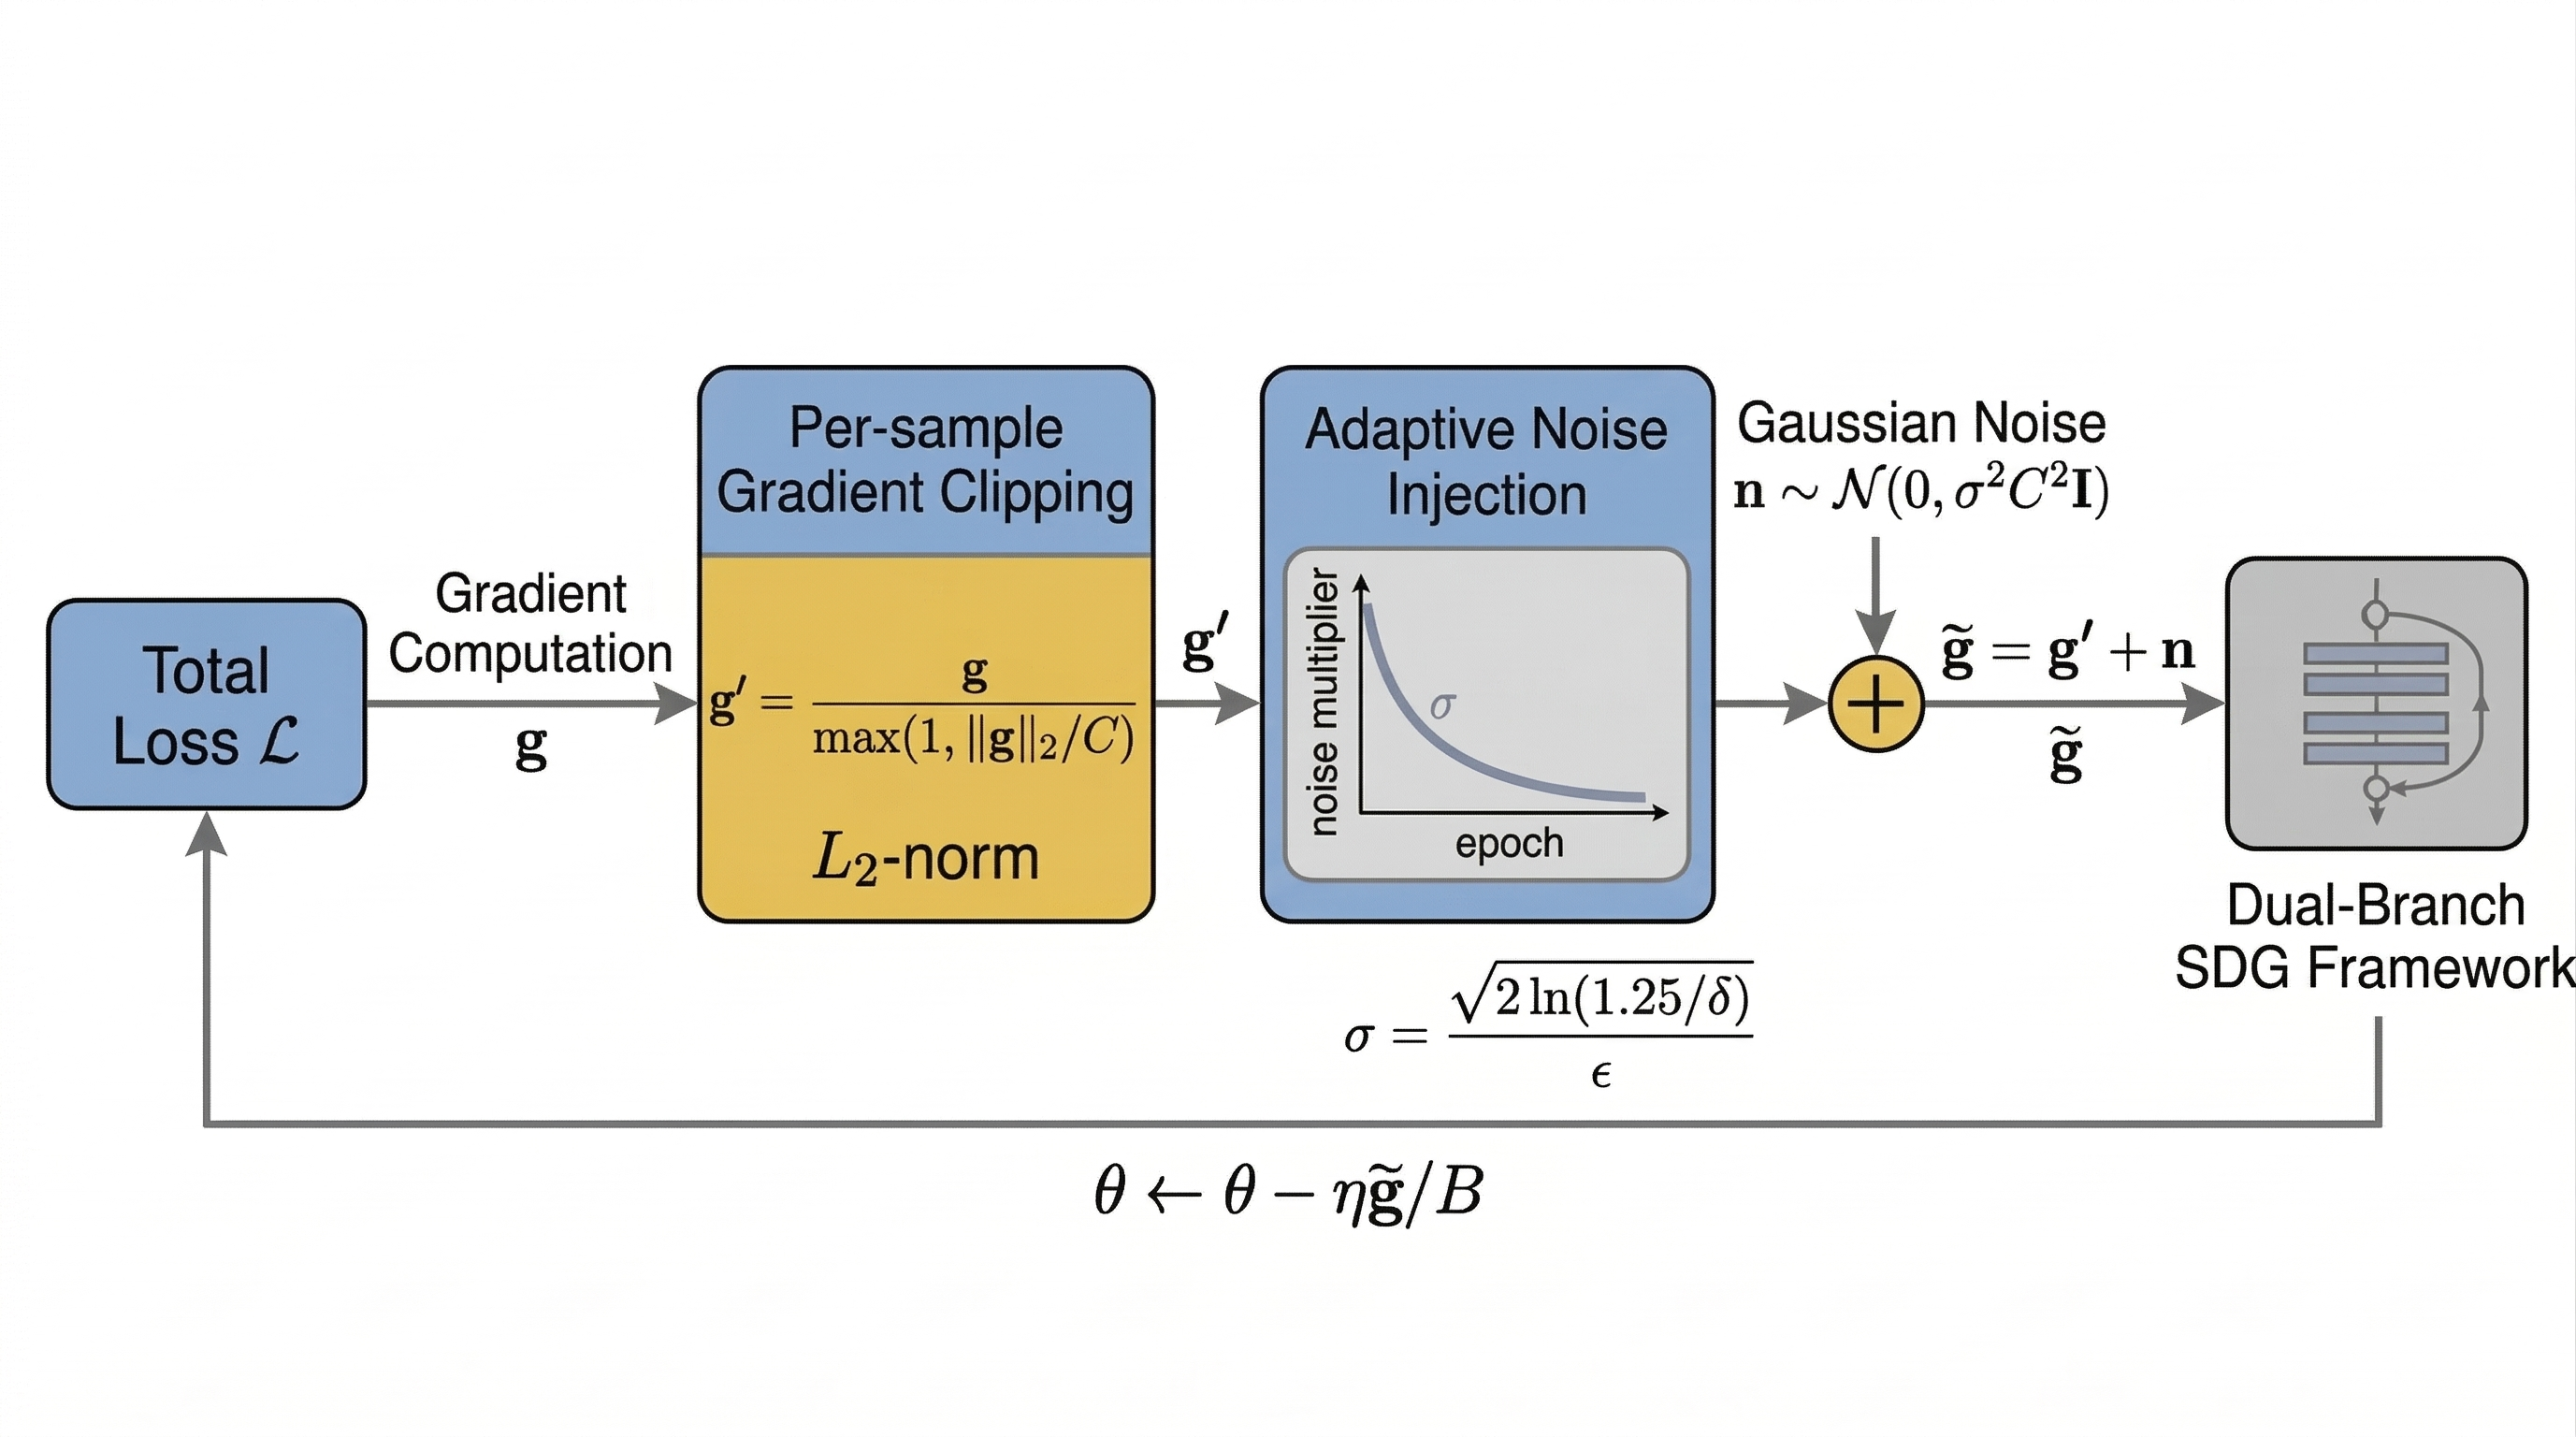
\includegraphics[width=5.74514in,height=3.13611in,alt={privacy-sdg}]{./images/media/image3_v2.png}

高斯差分隐私（Gaussian DP）通过在每步梯度更新时加入独立同分布的高斯噪声实现\((\epsilon, \delta)\)-差分隐私。对于相邻数据集\(D\)和\(D'\)（仅相差一个样本），若随机算法\(M\)对任意输出集合\(S\)满足：

\[\Pr\lbrack M(D) \in S\rbrack \leq e^{\epsilon}\Pr\lbrack M(D') \in S\rbrack + \delta,
\]

则称\(M\)满足\((\epsilon, \delta)\)-DP，其中\(\epsilon\)衡量隐私损失，\(\delta\)为松弛概率，通常设为\(10^{-5}\)。在DP-SGD框架下，每次迭代对每个样本梯度\(g\)先进行L2范数裁剪：

\[g' = g/max(1, \parallel g \parallel_{2}/C),
\]

然后加入高斯噪声\(n \sim \mathcal{N}(0,\sigma^{2}C^{2}I)\)，噪声方差\(\sigma\)由隐私预算决定：

\[\sigma = \sqrt{2\ln(1.25/\delta)}/\epsilon.
\]

噪声梯度\(\widetilde{g} = g' + n\)，更新\(\theta \leftarrow \theta - \eta\widetilde{g}/B\)，其中\(B\)是批次大小。该过程通过注入噪声模糊梯度，防止逆向攻击恢复原始图像或标签。有关隐私保护机制及其安全性的详细证明，请参阅Dwork C etal.\hyperref[_Ref214903493]{{[}48{]}}的工作。

然而，传统高斯DP在整个训练过程中使用固定\(\sigma\)，导致训练后期仍注入大量噪声，严重损害模型收敛和最终性能。为此，我们采用自适应高斯差分隐私优化器（AdaGaussian），其核心在于动态衰减噪声强度：训练初期使用较大噪声乘数以快速消耗隐私预算、提供强保护；随着模型逐渐收敛，根据预设衰减策略逐步降低噪声乘数，使后期扰动最小化，从而在相同最终\(\epsilon\)下显著提升模型可用性。由于噪声强度随训练动态衰减，该机制虽无法像固定噪声那样对每一轮提供严格的\(\epsilon\)会计，但整体仍能满足松弛的\((\epsilon, \delta)\)-差分隐私保证。最终实验验证，在确保中等隐私保护下，泛化性能可持平基线，验证了自适应高斯差分隐私在眼科多标签单域泛化任务中的优越性。

\subsection{4.实验}\label{ux5b9eux9a8c}

A．数据集

本实验主要采用ODIR-5K（Ocular Disease Intelligent Recognition）\hyperref[_Ref213949402]{{[}49{]}}数据集作为单域训练集。ODIR包含5000名患者的10000张彩色眼底图像（左右眼各5000张），由3名具有2年以上临床经验的眼科医生初步标注，并由3名10年以上经验的专家进行最终仲裁。数据集定义了8个互不排斥的类别：正常（N）、糖尿病视网膜病变（D）、青光眼（G）、白内障（C）、年龄相关性黄斑变性（A）、高血压视网膜病变（H）、病理性近视（M）和其他异常（O），\hl{如图4(a)到(h)所示}，属于典型的多标签分类任务。每张图像可能同时具有多个疾病标签，患者级标签由其左右眼诊断关键词综合确定。官方将5000名患者划分为3个子集，训练集（3500人）用于模型训练、offset测试集(500人)用于模型的选择，onset测试集(1000人)用于测试模型的泛化性能。各类别分布如表1所示，存在有类别不平衡问题。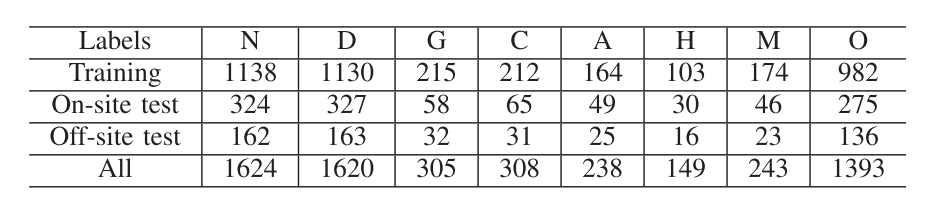
\includegraphics[width=5.76806in,height=1.31111in]{./images/media/image4.png}

为全面评估模型的单域泛化与跨域泛化能力，除ODIR同域测试外，我们额外引入RIADD挑战赛提供的RFMiD\hyperref[_Ref213949409]{{[}50{]}}数据集作为独立跨域测试集。RFMiD包含3200张彩色眼底图像，涵盖45种视网膜疾病或异常，由专业视网膜专家标注。其45类标签中含有部分与ODIR的8类标签重合的类别，这为模型泛化提供了基础，同时RFMiD与ODIR在成像设备、光照条件、患者种族等方面存在显著域差异，是检验单域泛化能力的优秀外部测试集，\hl{图5（a）到（h）选择性地展示了45种类别中的8类图像}。

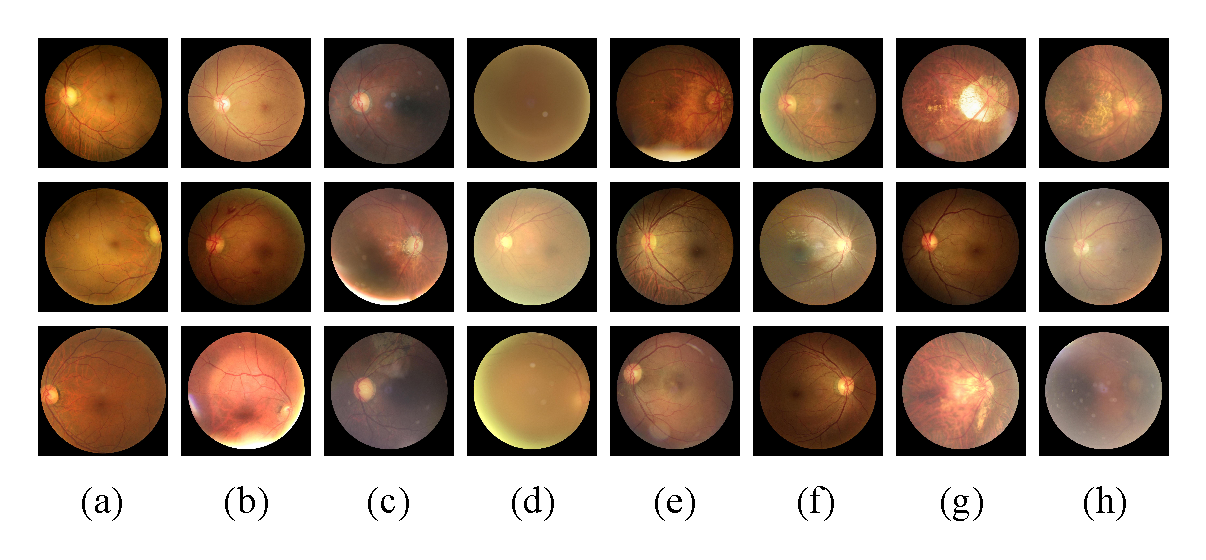
\includegraphics[width=5.76597in,height=2.52222in]{./images/media/image5_padded.pdf}

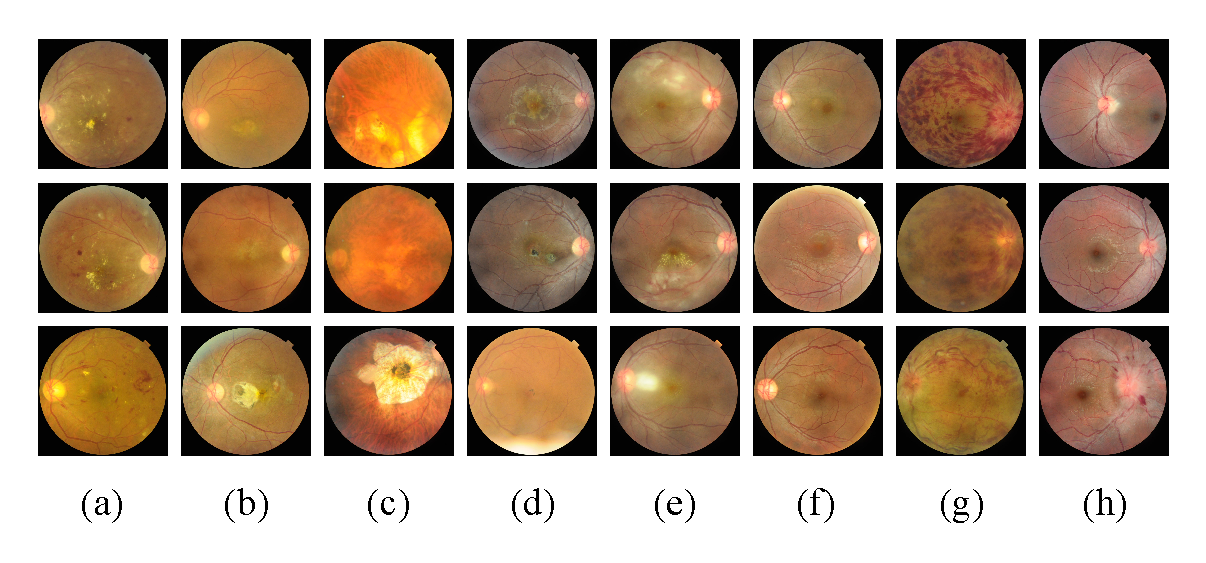
\includegraphics[width=5.75903in,height=2.49653in]{./images/media/image6_padded.pdf}

B．实验设置\\
所有实验均以ResNet-50作为骨干网络，并在PyTorch框架下实现。评估指标沿用ODIR官方标准：Kappa系数、F1、AUC以及三者平均值Final score。Kappa阈值固定为0.5，F1采用micro平均方式以缓和类别不平衡影响。

对于基准框架，我们参考ODIR原始的ResNet-50的实现，并在此基础上进行了改进：原论文采用双目样本成对输入，尝试不同的特征层融合策略（如concat、prod、sum）后接8个独立的分类头进行患者级预测。我们的基准框架改为单眼图像为输入样本，样本同时带有所属患者的编号，分类器统一为单个多标签分类头，输出8维logits后经Sigmoid激活得到各疾病概率，损失函数为标准二元交叉熵（BCE）。推理阶段，将同一患者左右眼的单眼预测结果按逻辑合并得到患者级预测，从而与官方指标完全对齐。该改进避免了特征融合带来的噪声放大和个体差异信息稀释，尤其在双眼病变程度不一致时更有优势。

训练配置如下：优化器选择Adam，初始学习率\(1 \times 10^{-5}\)，采用OneCycleLR调度策略（前10\%轮次线性升温至峰值\(1 \times 10^{-5}\)，有助于模型快速跳出局部最优，后90\%轮次退火，有助于收敛和找到更优解），训练epoch为50，batch size为32，输入分辨率为448×448。所提框架在2张RTX 4080 Super上完成训练。后续实验结果表明，我们的改进基准框架（Off-set双目Final score 75.45）比起ODIR原文实现（Offset-双目Final score 68.00）能达到更好的效果。

C．与现有方法对比

为评估所提方法在ODIR数据集上的分类性能，我们选取了四个典型的多标签眼科疾病分类方法，包括ODIR数据集论文提供的官方基线（Li et al\hyperref[_Ref213949402]{{[}49{]}}）以及三项后续工作（Gour and Khanna、He etal、Ou etal）。这些方法主要聚焦于提升Final score，未考虑跨域泛化或隐私保护。表7报告了在Off-set和On-set测试集上的双目指标的ours方法和各方法的对比。

Gour and Khanna\hyperref[_Ref214903299]{{[}51{]}}提出基于转移学习的CNN框架，骨干网络采用VGG16，通过数据增强方法扩充ODIR数据集，然后采用SGD优化器细调模型，焦点在于利用预训练权重捕捉血管、视盘、黄斑等结构异常，以提升多类共存场景的鲁棒性。

He et al.\hyperref[_Ref214903312]{{[}52{]}}开发密集相关网络（DCNet），包括骨干CNN提取双眼特征、空间相关模块捕捉像素级相关性，以及分类器生成患者级分数。核心原理是通过密集卷积块融合左右眼特征，建模DR与AMD等疾病共现，但需依赖双目输入。

Ou et al.\hyperref[_Ref214903327]{{[}53{]}}设计双流交互CNN，使用特征增强模块通过注意力机制捕捉双眼局部-全局依赖，并多尺度模块叠加不同分辨率特征以丰富表示。其原理在于利用双流交互强化病变区域（如微血管瘤、出血点），提升多标签预测，但未考虑隐私或跨域场景。

结果显示，所提方法在Off-set集的Final score为78.83，领先BFENet 0.83；在On-set集为76.76，领先BFENet 0.06。证明了双分支域不变提取与自适应标签关联构建的优越性。

除了性能领先，所提方法的核心优势其实在于单域泛化：仅在ODIR单域训练后，泛化到RFMiD上提升了3.65分，而对比方法未探索跨数据集鲁棒性；此外，我们探索出一套隐私加密条件下的泛化方案，在\(\epsilon \approx 10\)下性能下降10\%，持平ODIR基准，同时保留CAM图可视化带来的可解释性。这些额外贡献使框架更适用于临床部署，超越了对比方法的单一性能追求。

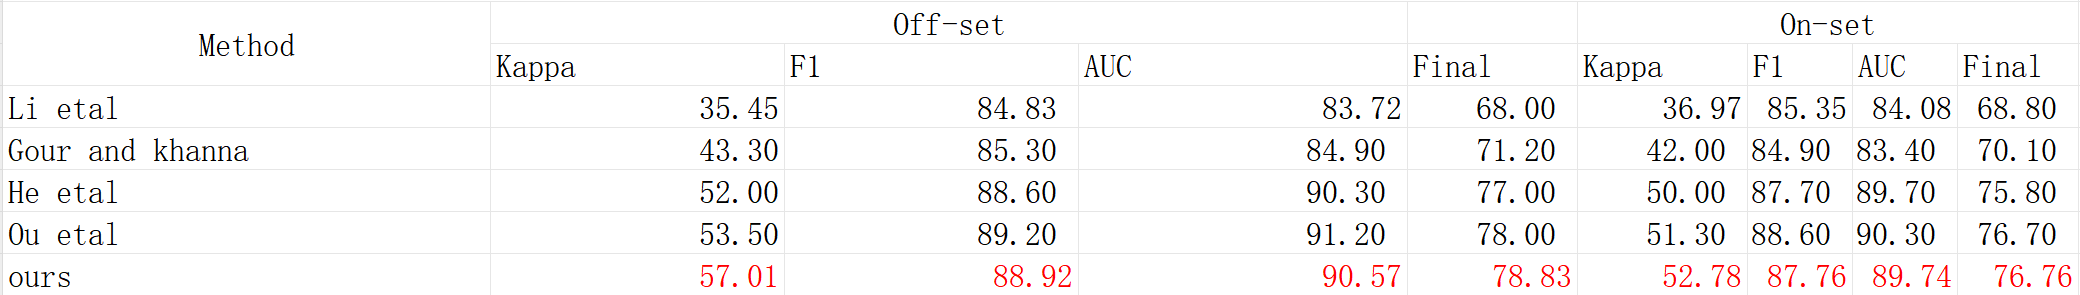
\includegraphics[width=5.76806in,height=0.81806in]{./images/media/image7.png}

D．消融实验结果\\
为系统验证所提框架中两大核心模块------双分支引导域不变特征提取（Dual-branch guided Domain-invariant Feature Extraction, DFE）与自适应标签-特征关联性构建（Adaptive label-feature Relevance Construction, ARC）的独立贡献及协同增益，同时考察CAM引导对模型可解释性的提升，我们在ODIR Off-set双目指标上进行了逐模块消融实验，结果如表6所示。

\begin{itemize}
\item
  纯ResNet-50基线：仅使用单分支ResNet-50与标准多标签分类头，Final score为75.45，Kappa为51.68。
\item
  ResNet50+DFE：仅引入完整的双分支引导域不变特征提取模块，Final score大幅提升至77.88（+2.43），Kappa提升3.33，AUC提升3.41。性能提升主要源于CAM引导残差加权与掩码机制有效抑制了域特定噪声，成功提取了对疾病更鲁棒的域不变特征，是泛化能力提升的最主要来源。\hl{如图6可视化结果显示，CAM热力图聚焦于图像边缘、光照伪影的概率降低，关注区域更收敛到眼球、血管等核心疾病区，模型可解释性增强}。
\item
  ResNet50+ARC：仅引入自适应标签-特征关联性构建模块，Final score提升至76.97（+1.52），Kappa提升1.50，AUC提升3.45。该模块通过显式建模疾病共现关系（如DR与AMD、近视与视盘异常）降低了漏检率，多标签分类性能提高。
\item
  ResNet50+DFE+ARC（完整框架，ours）：同时启用两大模块协同后，Final score进一步升至78.83（较基线+3.38），Kappa达到57.01（+5.33），F1与AUC分别达到88.92（+1.10）和90.57（+3.73）。总增益与两模块增益之和接近（3.38 \textless{} 2.43+1.52=3.95），体现了显著的正向协同：DFE为ARC提供纯净的域不变疾病特征，使Transformer能更精准地学习标签依赖与特征-标签匹配；ARC的一致性损失反过来进一步约束双分支输出分布，提升域不变特征稳定性。

  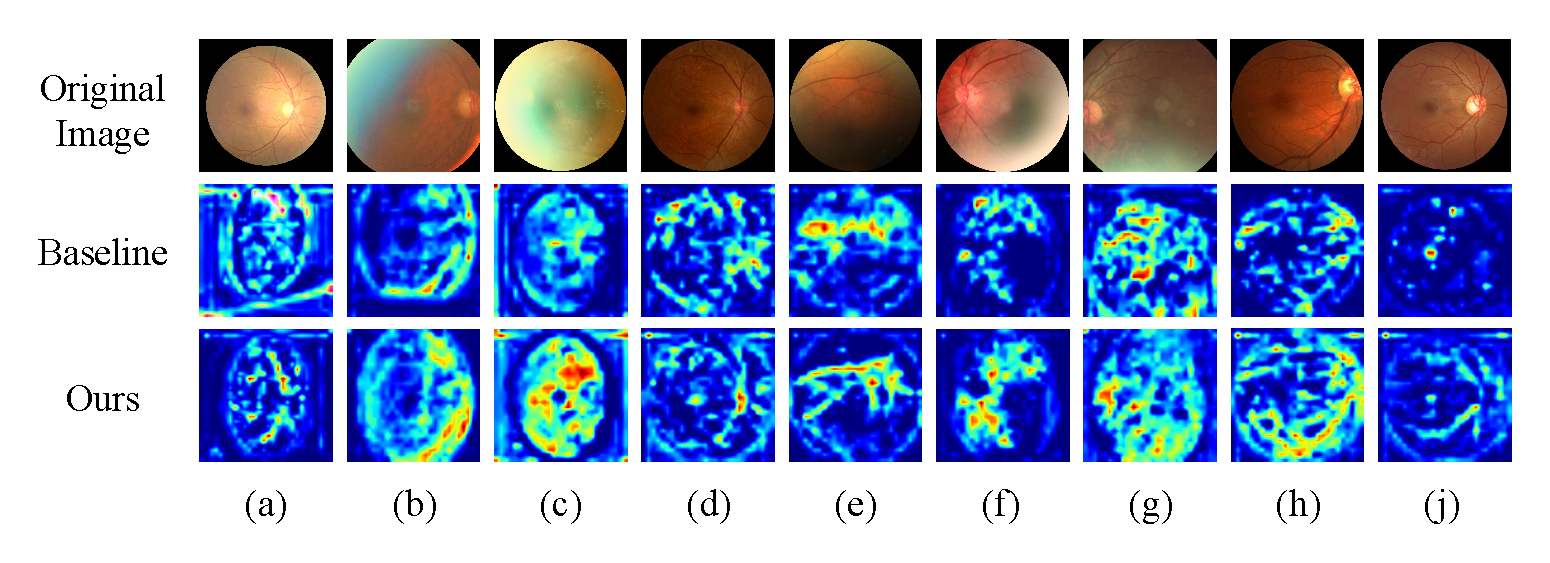
\includegraphics[width=5.75972in,height=1.96181in]{./images/media/image8_padded.pdf}
\end{itemize}

消融结果证明：双分支引导域不变特征提取（DFE）是框架泛化能力提升的主要来源，而自适应标签-特征关联性构建（ARC）在多标签共现建模与误检抑制方面发挥了不可替代的作用。两模块的深度融合协同使得所提框架在仅使用单域数据训练的情况下，性能进一步提升，体现了本方法设计的科学性与高效性。

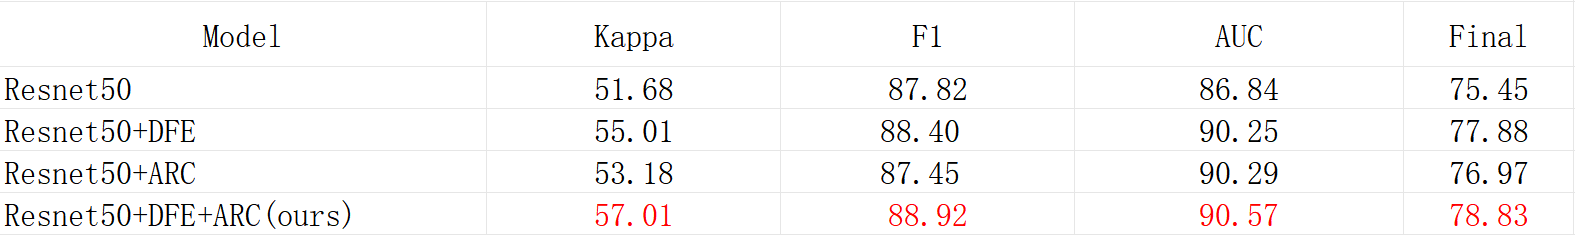
\includegraphics[width=5.76806in,height=0.86042in]{./images/media/image9.png}

E.泛化性能结果

为全面验证所提框架在单域训练条件下的泛化能力以及隐私保护机制的有效性，我们分别在非隐私和隐私保护两种场景下进行了系统性评估，涵盖同域测试（ODIR Off-set 与 On-set）和跨域测试（RFMiD）。

（1）非隐私条件下的泛化性能 表2报告了完整ODIR训练集（3500名患者）上训练后，基线与所提方法在不同测试集上的Final score。在同域Off-set和On-set测试集，我们同时报告单目（Monocular）和双目（Binocular）两种评估方式的结果。ResNet-50基线在两数据集下的双目指标分别为75.45和73.21，而所提方法将指标提升至78.83和76.76，增幅分别达3.38和3.55个百分点；单目指标提升更为明显（81.96 vs 79.08、78.44 vs 76.16），这得益于双分支域不变特征提取与CAM引导注意力对疾病区域的精准聚焦。其中双目指标低于单目指标的原因是，模型本身是以单目数据进行的训练，合并时若任一只眼出现预测异常就会判为患者有病，无论另一只眼结果如何，这会放大模型小错误的影响，导致整体指标下降，即可能出现原本单眼预测正确的情况，合并后因另一只眼预测不好而被拉低部分表现。

为进一步考察跨域泛化能力，我们提取ODIR与RFMiD共有的三类主要疾病（糖尿病视网膜病变DR、年龄相关性黄斑变性AMD、病理性近视），构建ODIR-3和RFMiD-3子集，仅在这三类上进行评估。原因在于RFMiD为单眼图像且包含大量ODIR未见类别，直接在完整8类上测试会导致标签空间不匹配：模型可能错误预测ODIR特有类（如青光眼、白内障）或无法识别RFMiD独有异常。通过限定为共有三类，可公平衡量模型对核心视网膜病变的跨域识别能力。结果显示，所提方法在RFMiD-3上取得68.49的Final score，较基线提升3.65个百分点，充分证明框架有效缓解了成像设备、光照条件、患者种族分布等因素带来的域偏移。

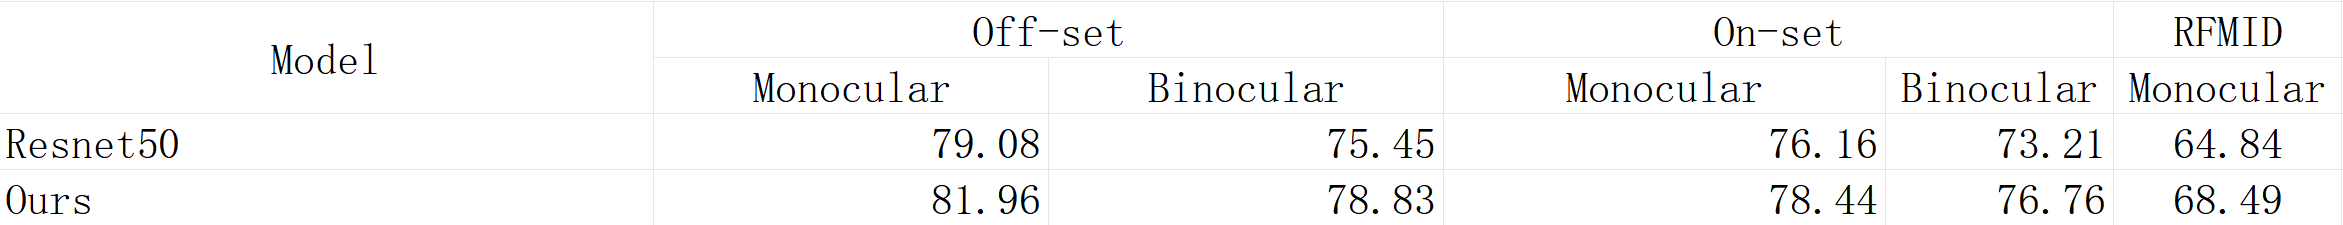
\includegraphics[width=5.76806in,height=0.55417in]{./images/media/image10.png}

（2）自适应高斯差分隐私超参数扫描 引入隐私保护后，噪声注入速率会一定程度影响模型收敛行为与最终性能。实验发现，初始噪声乘数（noise\_multiplier）与衰减速率（noise\_decay\_rate）共同决定了噪声注入曲线：过强的初始噪声会导致训练剧烈震荡甚至不收敛，而过快的衰减则使隐私预算在模型尚未充分学习时提前耗尽。表3展示了8组典型配置在固定80 epoch后的最终\(\epsilon\)值与收敛情况。其中，setting1（noise\_multiplier=0.65）提高了极强的隐私保护，但因初始噪声过大导致\(\epsilon\)仅5.01但模型性能会严重下滑；setting8（noise\_multiplier=0.25，decay\_rate=4e-6）虽然使得模型性能接近非隐私情况，但是\(\epsilon \approx 20\)隐私保护弱。综合性能与隐私预算，我们最终选取setting5（noise\_multiplier=0.35，decay\_rate=4e-6），在80 epoch后\(\epsilon \approx 10.15\)，实现了隐私强度与模型可用性的最佳折衷。

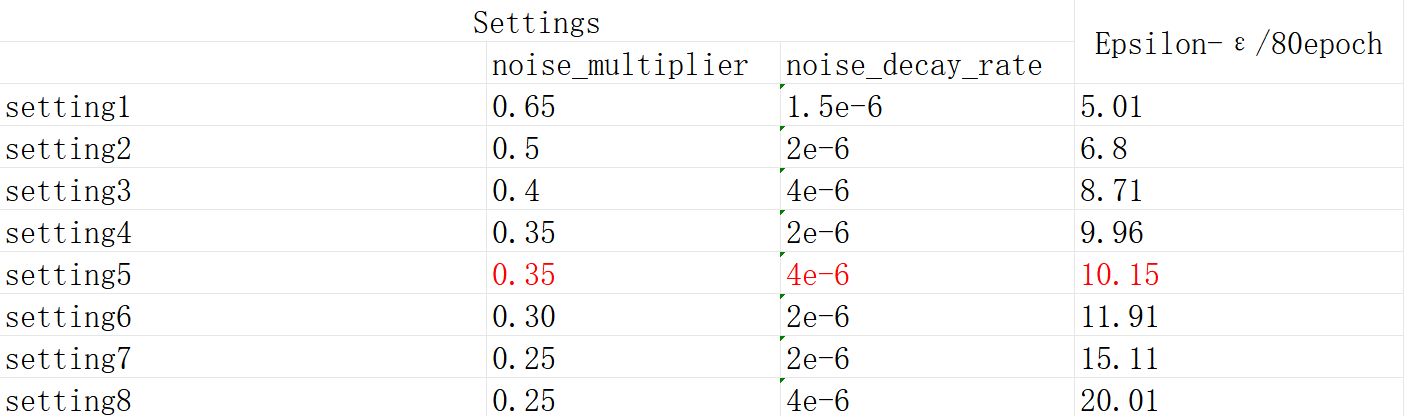
\includegraphics[width=5.76806in,height=1.70903in]{./images/media/image11.png}

（3）隐私训练过程中的\(\epsilon\)-性能演化与优化策略 采用setting5的噪声速率后，我们记录了训练过程中\(\epsilon\)消耗与单目指标的逐epoch变化（表4）。结果显示，随着\(\epsilon\)从第0轮的0.94逐步增长至第79轮的10.15，隐私逐步消耗，模型性能持续提升，至第74轮附近达到峰值（Final=73.15）。这表明自适应衰减策略允许模型在隐私预算内充分学习。取第74轮的模型权重是兼具隐私保护和性能的平衡点。经过大量实验验证，隐私场景需对优化策略进行针对性调整：

学习率从\(1 \times 10^{-5}\)提升至\(7.5 \times 10^{-5}\)

学习率调度改为``先线性衰减后恒定''： 以lr\_decay\_ratio和lr\_final\_factor控制衰减轮次和衰减比例，所取值分别为0.75和0.8，即学习率在前75\%轮次内线性衰减至原值的80\%，之后保持恒定训练。

原因在于，隐私情况下的模型训练和常规情况下的模型训练不一样。对于学习率的取值来说，隐私情况下，每一次回传的梯度中都会叠加噪声，这使得每一次模型优化时的损失值在原基础上波动，增大了陷入局部最优的概率，因此学习率需要适当增大。对于学习率调度策略，在常规情况下当模型收敛到最优值附近时，非隐私训练的学习速率通常会逐步减小；相比之下，隐私情况下的学习过程不需要将学习率降低到一个非常小的值，因为差分隐私训练会以隐私消耗不断增大的代价持续优化，却未必真正达到模型收敛。因此，以相对较大的学习率开始，然后在一定周期内线性衰减到较小的值，并在之后保持恒定，性能会更好。

实验证明，该策略改善了收敛稳定性，最终在\(\epsilon = 9.76\)时取得了73.15的Final score，明显优于固定噪声或低学习率配置。

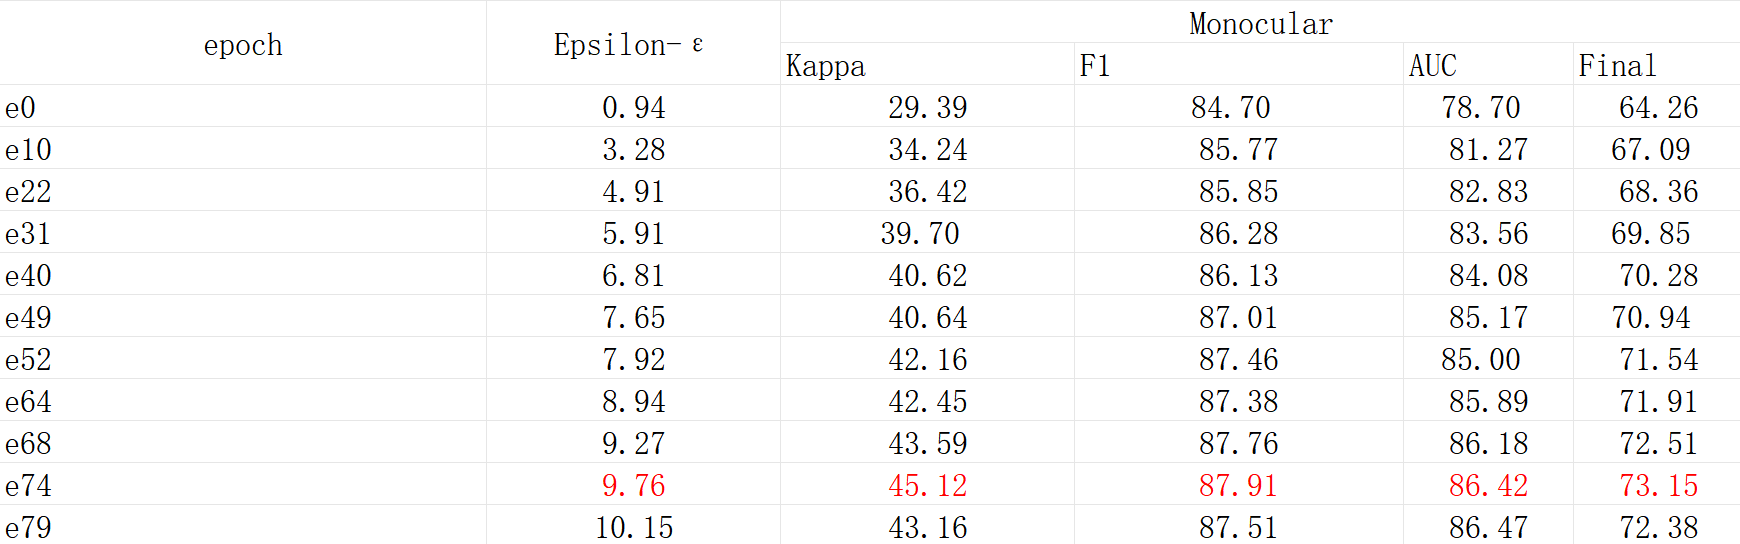
\includegraphics[width=5.76806in,height=1.80347in]{./images/media/image12.png}

（4）隐私保护下的最终泛化性能 表5报告了最优隐私模型在ODIR同域双目指标上的表现。Off-set和On-set的Final score分别为68.96和68.42，相较无隐私版本下降约10个百分点，但已接近或略优于ODIR原文官方基线（68.8），实现了在中等隐私预算下与公开基准持平的性能，充分体现了自适应高斯差分隐私机制的有效性。

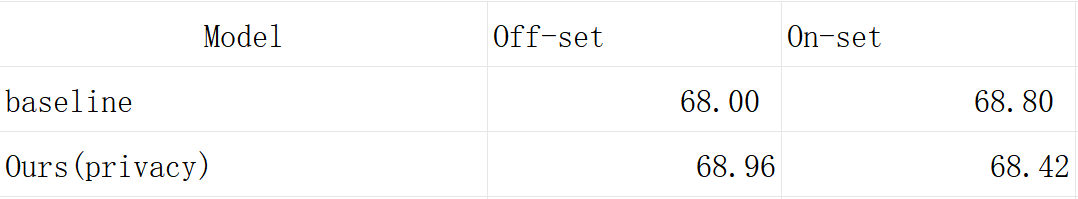
\includegraphics[width=5.76806in,height=1.06458in]{./images/media/image13.png}

\subsection{5.结论与讨论}\label{ux7ed3ux8bbaux4e0eux8ba8ux8bba}

本文提出了一种面向多标签眼科疾病分类的可解释与隐私保护单域泛化框架，针对传统方法在域偏移、多标签共现、和医疗隐私泄露等方面的局限性，提供了一个全面解决方案。核心贡献包括：（1）双分支引导域不变特征提取模块（DFE），通过风格增强模拟域偏移、CAM热图提供疾病区域先验引导，并结合空间/通道注意力与掩码过滤提取鲁棒特征，不仅提升了泛化性能，还增强了可解释性；（2）自适应标签-特征关联性构建模块（ARC），利用Transformer自/交叉注意力捕捉标签间依赖与特征-标签匹配，并通过一致性损失对齐双分支输出，显著减少多标签误检漏检；（3）自适应高斯差分隐私机制（AdaGDP），动态衰减噪声强度，在中等隐私预算（\(\epsilon \approx 10\)）下最小化性能损失，实现隐私-泛化兼顾。系统而完整的实验验证了所提出方法的有效性。尽管取得进展，本框架仍存在局限：对类别不平衡敏感，主体类（如DR、AMD）效果优异，但极小类别（如青光眼、白内障）易受影响，导致整体泛化受限，未来考虑用重采样或损失加权来缓解不平衡问题；当前泛化局限于共有类（如DR、AMD、近视），未来可探索分布外泛化以进一步提升性能。

\subsection{6.参考文献}\label{ux53c2ux8003ux6587ux732e}

\begin{enumerate}
\def\labelenumi{\arabic{enumi}.}
\item
  \protect\phantomsection\label{_Ref213871637}{}Kumar V, Singh R S, Rambabu M, et al. Deep learning for hyperspectral image classification: A survey{[}J{]}. Computer Science Review, 2024, 53: 100658.
\item
  \protect\phantomsection\label{_Ref213948625}{}Mo Y, Wu Y, Yang X, et al. Review the state-of-the-art technologies of semantic segmentation based on deep learning{[}J{]}. Neurocomputing, 2022, 493: 626-646.
\item
  \protect\phantomsection\label{_Ref213948646}{}Ramzan S, Iqbal M M, Kalsum T. Text-to-image generation using deep learning{[}J{]}. Engineering Proceedings, 2022, 20(1): 16.
\item
  \protect\phantomsection\label{_Ref213948898}{}Qiu D, Cheng Y, Wang X. Medical image super-resolution reconstruction algorithms based on deep learning: A survey{[}J{]}. Computer Methods and Programs in Biomedicine, 2023, 238: 107590.
\item
  \protect\phantomsection\label{_Ref213949262}{}Hasan S M M, Uddin M P, Al Mamun M, et al. A machine learning framework for early-stage detection of autism spectrum disorders{[}J{]}. IEEE Access, 2022, 11: 15038-15057.
\item
  \protect\phantomsection\label{_Ref213949290}{}Xuan P, Hu K, Cui H, et al. Learning multi-scale heterogeneous representations and global topology for drug-target interaction prediction{[}J{]}. IEEE Journal of Biomedical and Health Informatics, 2021, 26(4): 1891-1902.
\item
  \protect\phantomsection\label{_Ref213949294}{}Wang X, Wang F, Li Y, et al. Cxpmrg-bench: Pre-training and benchmarking for x-ray medical report generation on chexpert plus dataset{[}C{]}//Proceedings of the Computer Vision and Pattern Recognition Conference. 2025: 5123-5133.
\item
  \protect\phantomsection\label{_Ref213949315}{}Zhang W, Zhao X, Chen Y, et al. DeepUWF: an automated ultra-wide-field fundus screening system via deep learning{[}J{]}. IEEE Journal of Biomedical and Health Informatics, 2020, 25(8): 2988-2996.
\item
  \protect\phantomsection\label{_Ref213949336}{}Deng J, Dong W, Socher R, et al. Imagenet: A large-scale hierarchical image database{[}C{]}//2009 IEEE conference on computer vision and pattern recognition. Ieee, 2009: 248-255.
\item
  \protect\phantomsection\label{_Ref213949340}{}Lin T Y, Maire M, Belongie S, et al. Microsoft coco: Common objects in context{[}C{]}//European conference on computer vision. Cham: Springer International Publishing, 2014: 740-755.
\item
  \protect\phantomsection\label{_Ref213949348}{}Liu S, Yin S, Qu L, et al. Reducing domain gap in frequency and spatial domain for cross-modality domain adaptation on medical image segmentation{[}C{]}//Proceedings of the AAAI conference on artificial intelligence. 2023, 37(2): 1719-1727.
\item
  \protect\phantomsection\label{_Ref213949354}{}Yang C, Guo X, Chen Z, et al. Source free domain adaptation for medical image segmentation with fourier style mining{[}J{]}. Medical Image Analysis, 2022, 79: 102457.
\item
  \protect\phantomsection\label{_Ref213949362}{}Al-Fahdawi S, Al-Waisy A S, Zeebaree D Q, et al. Fundus-deepnet: Multi-label deep learning classification system for enhanced detection of multiple ocular diseases through data fusion of fundus images{[}J{]}. Information Fusion, 2024, 102: 102059.
\item
  \protect\phantomsection\label{_Ref213949382}{}Chen Z M, Wei X S, Wang P, et al. Multi-label image recognition with graph convolutional networks{[}C{]}//Proceedings of the IEEE/CVF conference on computer vision and pattern recognition. 2019: 5177-5186.
\item
  \protect\phantomsection\label{_Ref213949393}{}Bertino E, Ooi B C, Yang Y, et al. Privacy and ownership preserving of outsourced medical data{[}C{]}//21st International Conference on Data Engineering (ICDE\textquotesingle05). IEEE, 2005: 521-532.
\item
  \protect\phantomsection\label{_Ref213949439}{}Guan H, Liu M. Domain adaptation for medical image analysis: a survey{[}J{]}. IEEE Transactions on Biomedical Engineering, 2021, 69(3): 1173-1185.
\item
  \protect\phantomsection\label{_Ref213949448}{}Tzeng E, Hoffman J, Zhang N, et al. Deep domain confusion: Maximizing for domain invariance{[}J{]}. arXiv preprint arXiv:1412.3474, 2014.
\item
  \protect\phantomsection\label{_Ref213949453}{}Sun B, Feng J, Saenko K. Return of frustratingly easy domain adaptation{[}C{]}//Proceedings of the AAAI conference on artificial intelligence. 2016, 30(1).
\item
  \protect\phantomsection\label{_Ref213949479}{}Ganin Y, Ustinova E, Ajakan H, et al. Domain-adversarial training of neural networks{[}J{]}. Journal of machine learning research, 2016, 17(59): 1-35.
\item
  \protect\phantomsection\label{_Ref213949490}{}Zhu J Y, Park T, Isola P, et al. Unpaired image-to-image translation using cycle-consistent adversarial networks{[}C{]}//Proceedings of the IEEE international conference on computer vision. 2017: 2223-2232.
\item
  \protect\phantomsection\label{_Ref213949530}{}Wang R, Wu Z, Weng Z, et al. Cross-domain contrastive learning for unsupervised domain adaptation{[}J{]}. IEEE Transactions on Multimedia, 2022, 25: 1665-1673.
\item
  \protect\phantomsection\label{_Ref213949554}{}Zhou K, Liu Z, Qiao Y, et al. Domain generalization: A survey{[}J{]}. IEEE transactions on pattern analysis and machine intelligence, 2022, 45(4): 4396-4415.
\item
  \protect\phantomsection\label{_Ref213949562}{}Zhou K, Yang Y, Qiao Y, et al. Domain generalization with mixstyle{[}J{]}. arXiv preprint arXiv:2104.02008, 2021.
\item
  \protect\phantomsection\label{_Ref213949607}{}Gulrajani I, Lopez-Paz D. In search of lost domain generalization{[}J{]}. arXiv preprint arXiv:2007.01434, 2020.
\item
  \protect\phantomsection\label{_Ref213949788}{}Xu Q, Zhang R, Zhang Y, et al. A fourier-based framework for domain generalization{[}C{]}//Proceedings of the IEEE/CVF conference on computer vision and pattern recognition. 2021: 14383-14392.
\item
  \protect\phantomsection\label{_Ref213949796}{}Huang Z, Wang H, Xing E P, et al. Self-challenging improves cross-domain generalization{[}C{]}//European conference on computer vision. Cham: Springer International Publishing, 2020: 124-140.
\item
  \protect\phantomsection\label{_Ref213949803}{}Domain Generalization through Meta-Learning: A Survey
\item
  \protect\phantomsection\label{_Ref213949863}{}Ouyang C, Chen C, Li S, et al. Causality-inspired single-source domain generalization for medical image segmentation{[}J{]}. IEEE Transactions on Medical Imaging, 2022, 42(4): 1095-1106.
\item
  \protect\phantomsection\label{_Ref213949872}{}Wang Y, Xie Y, Fan L, et al. STMG: Swin transformer for multi-label image recognition with graph convolution network{[}J{]}. Neural Computing and Applications, 2022, 34(12): 10051-10063.
\item
  \protect\phantomsection\label{_Ref213949896}{}Zhang M L, Li Y K, Liu X Y, et al. Binary relevance for multi-label learning: an overview{[}J{]}. Frontiers of Computer Science, 2018, 12(2): 191-202.
\item
  \protect\phantomsection\label{_Ref213949927}{}Ridnik T, Ben-Baruch E, Zamir N, et al. Asymmetric loss for multi-label classification{[}C{]}//Proceedings of the IEEE/CVF international conference on computer vision. 2021: 82-91.
\item
  \protect\phantomsection\label{_Ref213950246}{}Liu S, Zhang L, Yang X, et al. Query2label: A simple transformer way to multi-label classification{[}J{]}. arXiv preprint arXiv:2107.10834, 2021.
\item
  \protect\phantomsection\label{_Ref213950282}{}Everingham M, Van Gool L, Williams C K I, et al. The pascal visual object classes (voc) challenge{[}J{]}. International journal of computer vision, 2010, 88(2): 303-338.
\item
  \protect\phantomsection\label{_Ref213950338}{}Shi M, Tang Y, Zhu X, et al. Multi-label graph convolutional network representation learning{[}J{]}. IEEE Transactions on Big Data, 2020, 8(5): 1169-1181.
\item
  \protect\phantomsection\label{_Ref213950343}{}Merlin R, Lloyd F V. An Efficient Model for Multi-Label Ocular Disease Classification using Fundus Images based on Attention-based Multiscale MobileNet{[}C{]}//2025 8th International Conference on Computing Methodologies and Communication (ICCMC). IEEE, 2025: 1083-1090.
\item
  \protect\phantomsection\label{_Ref213950349}{}Sun Z, Wu N, Shi J, et al. Fedmlp: Federated multi-label medical image classification under task heterogeneity{[}C{]}//International Conference on Medical Image Computing and Computer-Assisted Intervention. Cham: Springer Nature Switzerland, 2024: 394-404.
\item
  \protect\phantomsection\label{_Ref213950358}{}Yadav N, Pandey S, Gupta A, et al. Data privacy in healthcare: in the era of artificial intelligence{[}J{]}. Indian Dermatology Online Journal, 2023, 14(6): 788-792.
\item
  \protect\phantomsection\label{_Ref213950376}{}Aledhari M, Razzak R, Parizi R M, et al. Federated learning: A survey on enabling technologies, protocols, and applications{[}J{]}. IEEE Access, 2020, 8: 140699-140725.
\item
  \protect\phantomsection\label{_Ref213950381}{}Nguyen D C, Ding M, Pathirana P N, et al. Federated learning for COVID-19 detection with generative adversarial networks in edge cloud computing{[}J{]}. IEEE Internet of Things Journal, 2021, 9(12): 10257-10271.
\item
  \protect\phantomsection\label{_Ref213950391}{}Li T, Sahu A K, Zaheer M, et al. Federated optimization in heterogeneous networks{[}J{]}. Proceedings of Machine learning and systems, 2020, 2: 429-450.
\item
  \protect\phantomsection\label{_Ref213950427}{}Martins P, Sousa L, Mariano A. A survey on fully homomorphic encryption: An engineering perspective{[}J{]}. ACM Computing Surveys (CSUR), 2017, 50(6): 1-33.
\item
  \protect\phantomsection\label{_Ref213950433}{}Dutil F, See A, Di Jorio L, et al. Application of homomorphic encryption in medical imaging{[}J{]}. arXiv preprint arXiv:2110.07768, 2021.
\item
  \protect\phantomsection\label{_Ref213950438}{}Zhao C, Zhao S, Zhao M, et al. Secure multi-party computation: theory, practice and applications{[}J{]}. Information Sciences, 2019, 476: 357-372.
\item
  \protect\phantomsection\label{_Ref213950443}{}Bu Z, Dong J, Long Q, et al. Deep learning with gaussian differential privacy{[}J{]}. Harvard data science review, 2020, 2020(23): 10.1162/99608f92. cfc5dd25.
\item
  \protect\phantomsection\label{_Ref213950449}{}Dong J, Roth A, Su W J. Gaussian differential privacy{[}J{]}. Journal of the Royal Statistical Society Series B: Statistical Methodology, 2022, 84(1): 3-37.
\item
  \protect\phantomsection\label{_Ref213950453}{}Sabt M, Achemlal M, Bouabdallah A. Trusted execution environment: What it is, and what it is not{[}C{]}//2015 IEEE Trustcom/BigDataSE/Ispa. IEEE, 2015, 1: 57-64.
\item
  \protect\phantomsection\label{_Ref213950458}{}Bagdasaryan E, Poursaeed O, Shmatikov V. Differential privacy has disparate impact on model accuracy{[}J{]}. Advances in neural information processing systems, 2019, 32.
\item
  \protect\phantomsection\label{_Ref214903493}{}Dwork C, McSherry F, Nissim K, et al. Calibrating noise to sensitivity in private data analysis{[}C{]}//Theory of cryptography conference. Berlin, Heidelberg: Springer Berlin Heidelberg, 2006: 265-284.
\item
  \protect\phantomsection\label{_Ref213949402}{}Li N, Li T, Hu C, et al. A benchmark of ocular disease intelligent recognition: One shot for multi-disease detection{[}C{]}//International symposium on benchmarking, measuring and optimization. Cham: Springer International Publishing, 2020: 177-193.
\item
  \protect\phantomsection\label{_Ref213949409}{}Pachade S, Porwal P, Thulkar D, et al. Retinal fundus multi-disease image dataset (rfmid): A dataset for multi-disease detection research{[}J{]}. Data, 2021, 6(2): 14.
\item
  \protect\phantomsection\label{_Ref214903299}{}Gour N, Khanna P. Multi-class multi-label ophthalmological disease detection using transfer learning based convolutional neural network{[}J{]}. Biomedical signal processing and control, 2021, 66: 102329.
\item
  \protect\phantomsection\label{_Ref214903312}{}He J, Li C, Ye J, et al. Multi-label ocular disease classification with a dense correlation deep neural network{[}J{]}. Biomedical Signal Processing and Control, 2021, 63: 102167.
\item
  \protect\phantomsection\label{_Ref214903327}{}Ou X, Gao L, Quan X, et al. BFENet: A two-stream interaction CNN method for multi-label ophthalmic diseases classification with bilateral fundus images{[}J{]}. Computer Methods and Programs in Biomedicine, 2022, 219: 106739.
\end{enumerate}
